\documentclass{article}
\usepackage[utf8]{inputenc}
\usepackage{graphicx}
 \usepackage{gensymb}
\title{Lab 1: Photon Counting \& the Statistics of Light}
\author{Jung Lin (Doris) Lee}
\date{September 2014}

\begin{document}
\maketitle

\section{Introduction\label{intro}}
\indent Photon statistics are the fundamental basis to optical astronomy since they constitut e what 
are important to astronomy because 
optical astronomy 
galaxy morphology, 
Large sky surveys such as the Sloan Digital Sky Survey and the Dark Energy Survey   imaging data in the optical wavelength
\indent In this experiment, we recorded the arrival of photons from an LED and analyze
 In section 2, I will describe the experimental method that my group used to take the data and the results that we obtained. Subsequently, section 3 introduces the various statistical measures that we can use to describe the findings and observation on  a single dataset, including the effect of binning the data into histograms. Section 4 describes the two probability density functions that are relavant to these histograms and dataset.
\section{Experiments\label{experiment}}
	\subsection{Methods}
The arrival of a photon is registered by the photomultiplier tube (PMT) , data acquisition is conducted by the CoinPro software
% describe afterpulse and how to remove them;Measures taken to alleviate systematics effects 
Sometimes afterpulses can seen immediately after the original pulse.  We eliminate this systematic effects by cutting away 

\begin{figure}[h]
\centering
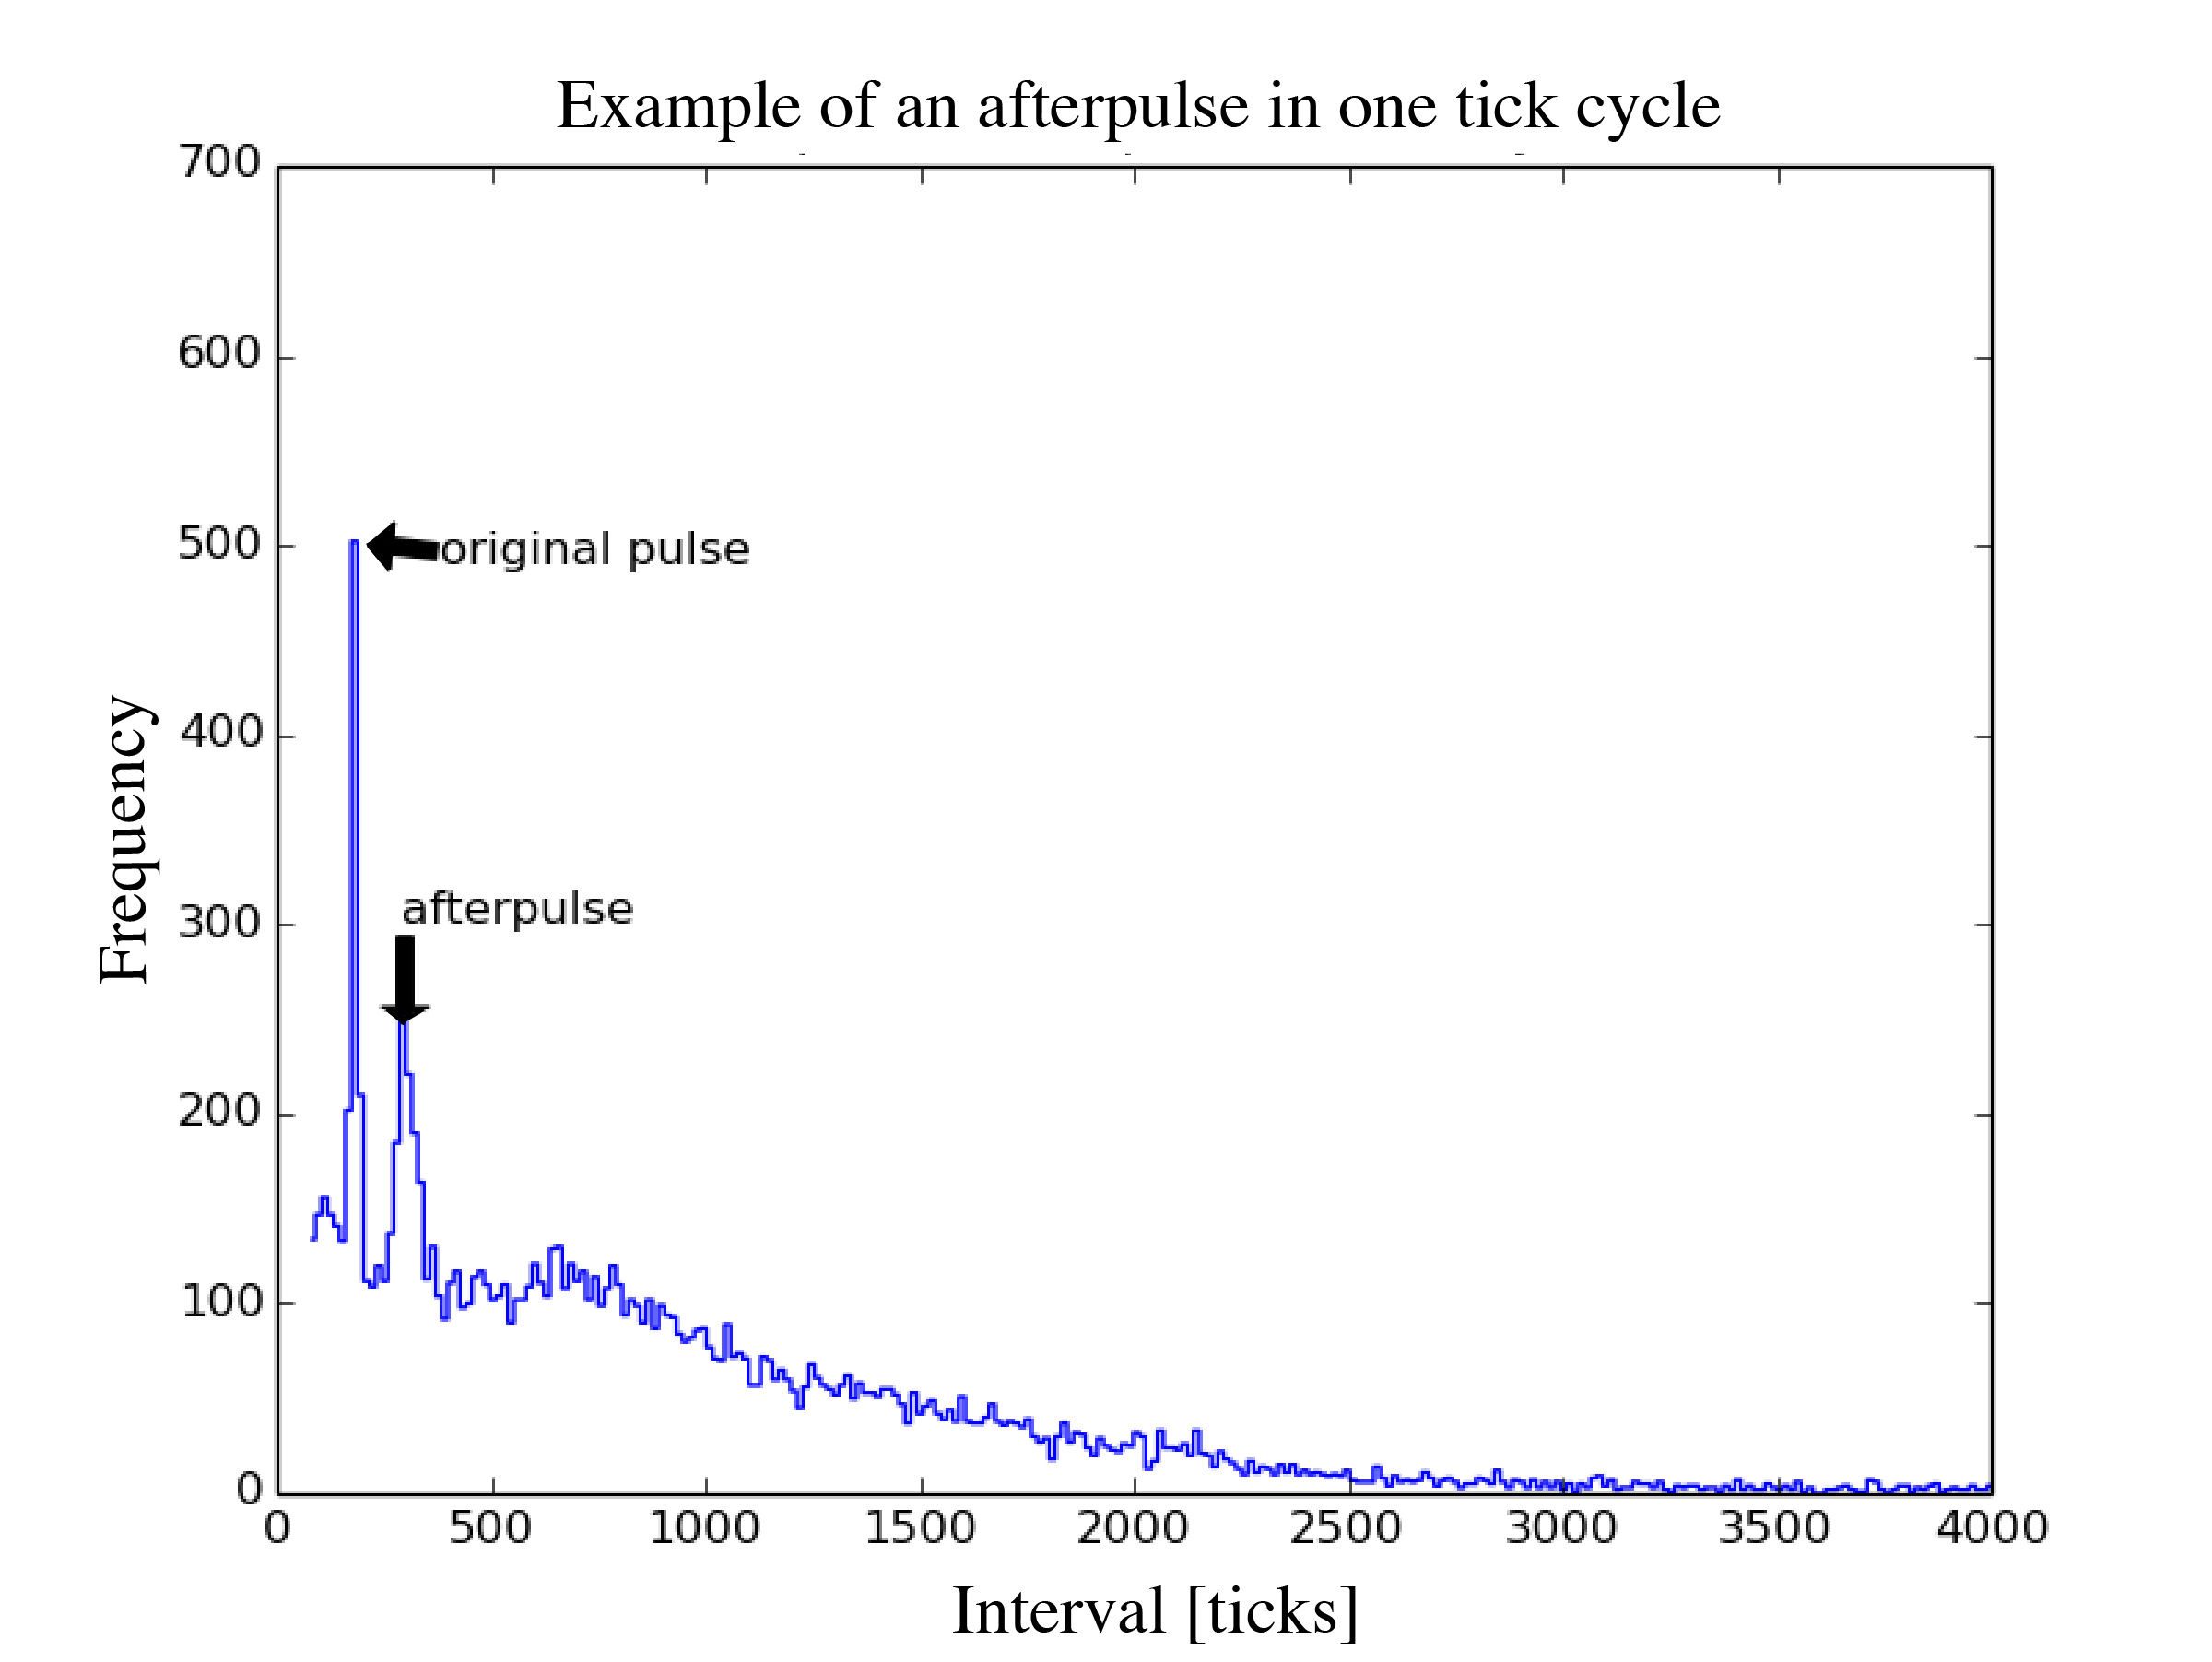
\includegraphics[width=0.8\textwidth]{figures/afterpulse}
\caption{The two peaks can be seen  there is a gradual decline of ticks in the next ~3000 clock ticks.}
\label{afterpulse}
\end{figure}
   \subsection{Changing LED Brightness}
\indent By listening to ticks on the squawker, there was no detectable difference from the 3 o'clock off position to the 12 o'clock position. Therefore, we started off at the 12 o'clock location and went to the max location ($\approx$90\degree), diving this region into 6 equal parts \footnote{Although it seems like only 5 data points are shown in the plot, this is merely an artifact of the choice of data representation as circles as  the first two data points lie so closely that they are almost indistinguishable. This is easily verified by using the dot representation with \texttt{matplotlib's} `,`setting} is roughly 15\degree  increments. Even though the measurement of the LED brightness is eyeballed and not that precise, it did not significantly affect the plot since the relation is linear . No matter what the brightness is, in theory, the data point should always follow the slope =1 linear relation.
\begin{figure}[h]
\centering
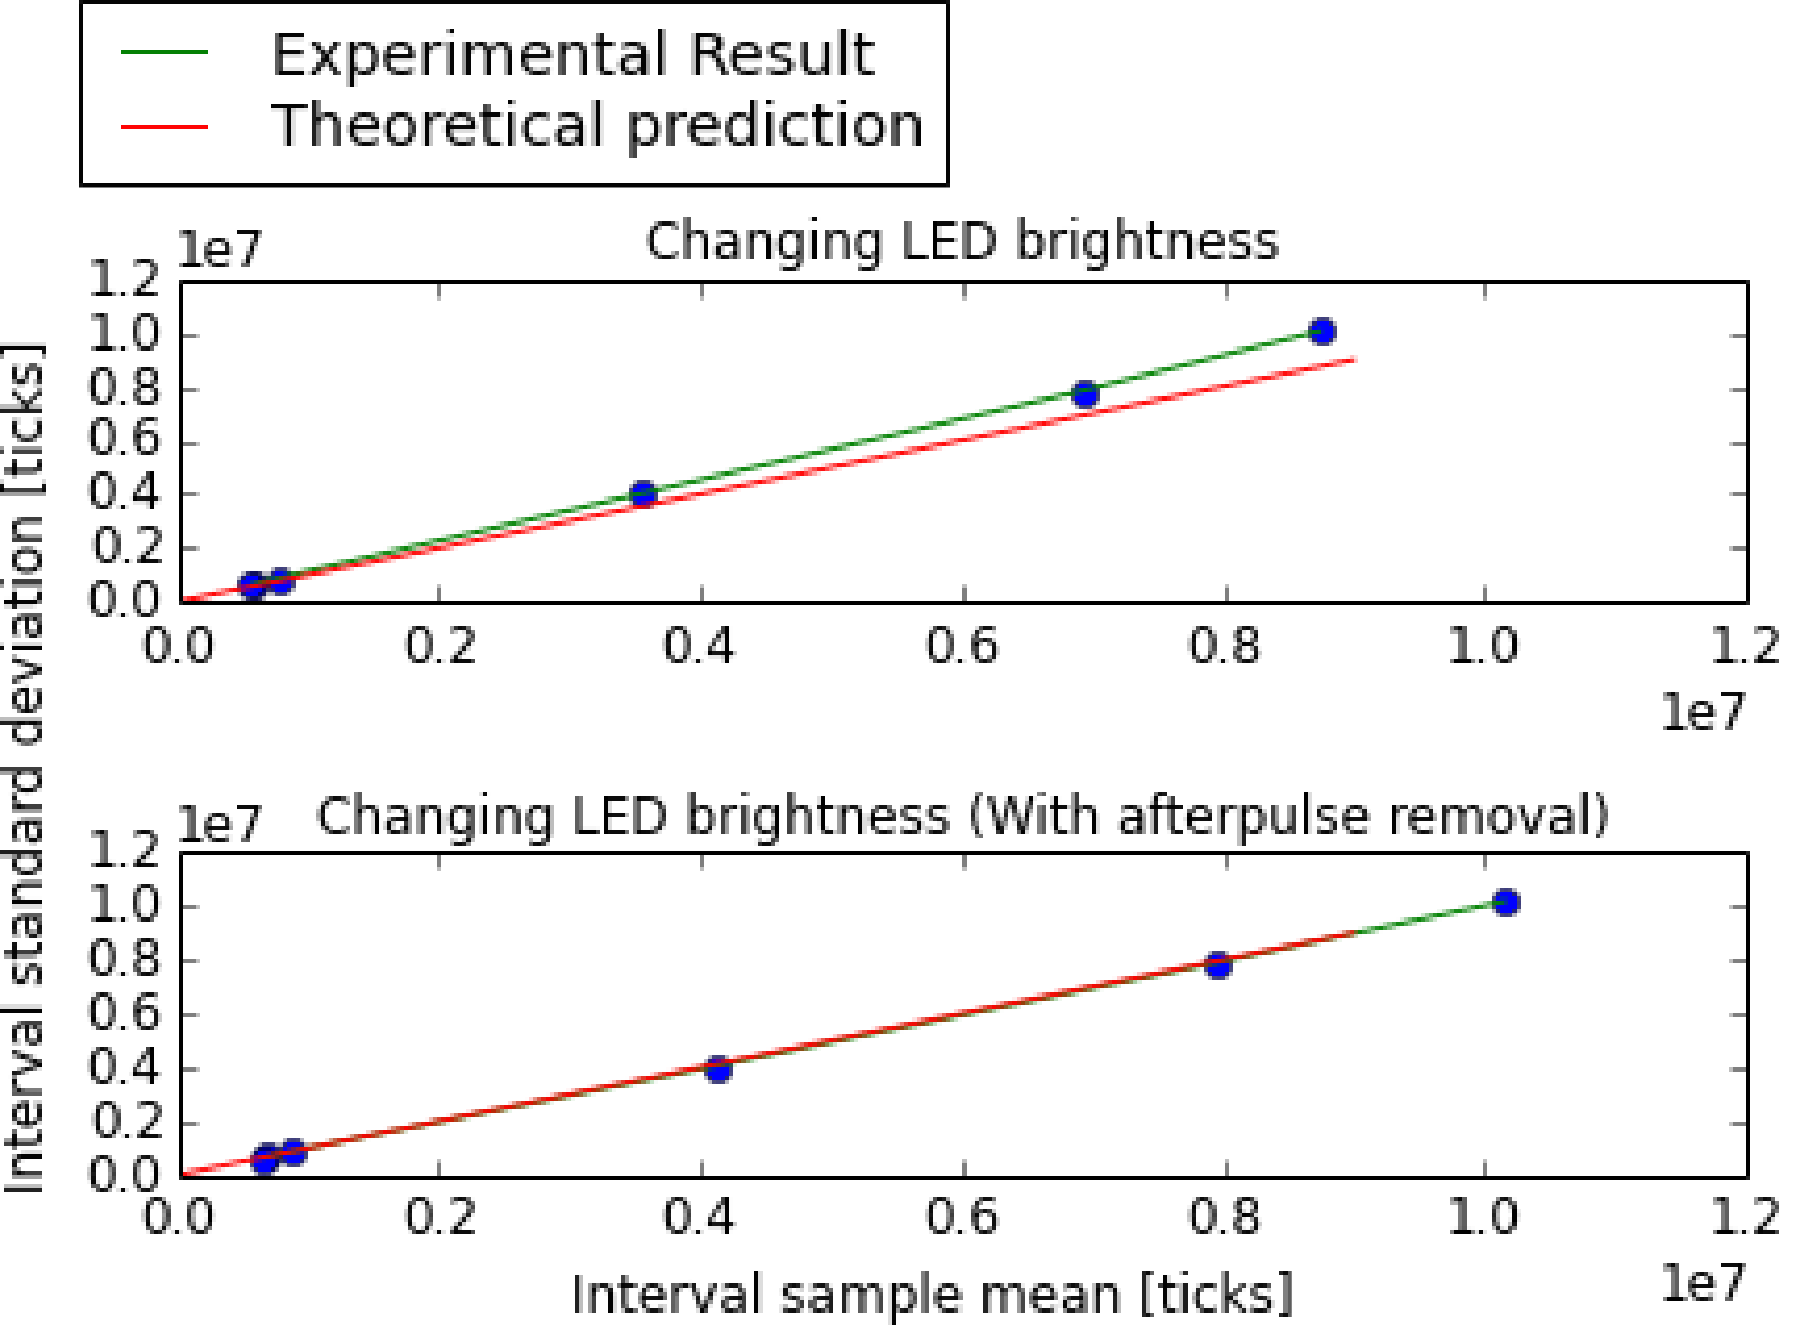
\includegraphics[width=0.8\textwidth]{figures/changeLED}
\caption{Showing linear relation between standard deviation and sample mean. The slope of the line should one since both the standard deviation and the sample mean of each dataset is equal to the single-parameter that governs the behavior of the exponential distribution.}
\label{changeLED}
\end{figure}
\section{Descriptive Statistics and Histograms\label{stats}}

\section{Photon Statistics\label{pstats}}
 	\subsection{Exponential Distribution}
 	\subsection{Poisson Distribution}
 	Unlike the continuous exponential distribution, Poisson dsitribution is a discrete probability distribution that arise from (\_). The underllying process is the same (rare event for very large N) btu the experiement method is different. In our case the wayh we post-process the data is different.
\section{Conclusion\label{end}}

\end{document}
